
\documentclass[a4paper,english]{IEEEtran}
\usepackage[T1]{fontenc}
\usepackage[latin9]{inputenc}
\usepackage{graphicx}

\usepackage[unicode=true, pdfusetitle,
 bookmarks=true,bookmarksnumbered=false,bookmarksopen=false,
 breaklinks=false,pdfborder={0 0 1},backref=false,colorlinks=false]{hyperref}

\makeatother

\usepackage{babel}

\begin{document}

\date{December 2011}

\author{Alexandre Chappuis, Bastian Marquis and David Klopfenstein @ EPFL.ch}

\title{Implementation of a BGP Route Flap Damping Algorithm for the Bird
Routing Project}

\maketitle

\begin{abstract}
Today's Internet stability strongly relies on the good behavior of
dynamic routing protocols such as BGP (Border Gateway Protocol), that
enables routing between Autonomous Systems. Route flapping is a well-known
and undesirable phenomenon occuring in both commercial and private
networks. In this report, we explain our implementation of the RFC
2439, BGP Route Flap Damping, for one famous Open Source routing software
suite, the Bird Routing Project.

We also present results of an experiment where we compared the number
of BGP updates sent with and without route damping enabled, in a setup
where only one of the bgp router was receiving advertisments for flapping
routes. 
\end{abstract}

\section{Introduction}

The inter-domain routing protocol BGP is still surviving to the gigantic
growth of the Internet that started during the last decade. However,
some widely used applications, such as Skype, still suffer from weaknesses
of that protocol. The main problems are twofolds: Firstly, BGP has
a slow convergence rate, meaning that a change at one location takes
quite some time to be propagated to the other ends of the network.
Secondly, if a node becomes unstable, for example if its connectivity
constantly comes up and down, it will have bad consequences on the
network, both in terms of useless processing at BGP routers and unnecessary
routing traffic. Routes advertised and withdrawn at regular interval
of time are said to be \textit{flapping}.

Many approaches to counter route flapping have been developped in
the late 90's. RFC 2439\cite{rfc2439} standardized one such approach
: it basically blocks updates from flapping routes, and does so until
the routes are deemed stable again. This RFC has been used it extensively
for many years, in both commercial and open source routers.

Although this standard is not recommended anymore\cite{ripe recommendations}
in today's routers, we wanted to implement it for the Bird Routing
Project\cite{bird}, hoping that it will serve as a good basis for
future possible improvements and extensions to this RFC. There exist
many variants of the Route Flap Damping alorithm and the community
has not lost its interest in finding robust mechanisms that could
allow BGP to be more resilient.


\section{Overview}

RFC 2349 seeks to limit the impact of route flapping by {}``damping''
(\textit{i.e.} ignoring packets of) missbehaving routes. The solution
must be able to distinguish flapping routes from good routes, consume
few resources, both in terms of memory usage and process time. The
RFC solves these problems by assigning each route a penalty term.
Whenever this penalty term for a given route reaches a certain threshold,
further advertisements for that route are ignored. This penalty term
varies over time : it is increased when the route becomes unreachable
and decays as long as the route stays stable. As soon as the figure
of merit goes below a \textit{reuse threshold}, the route can be used
again.

The figure of merits decays exponentially over time. Exponential decay
has several advantages : it can be implemented very efficiently using
precomputed \textit{decay arrays}. Also, with exponential decay, the
figure of merit keeps trace of previous instabilities for a fairly
long time : old instabilities become less and less important over
time, while newer ones have more weight.

Network administrators have lots of freedom in choosing the behavior
of the penalty term : they can control the half-life of the penalty
term, its maximum value (thus controlling the maximum time a route
can be suppressed) and both the reuse and cut thresholds.

Here is an example showing how the figure of merit evolves over time
(the illustration comes from \cite{damping-pic}). The route flaps
three times, exceeding the cut threshold only after the third flap.
The route is reused as soon as its penalty term goes below the reuse
limit.

\begin{center}
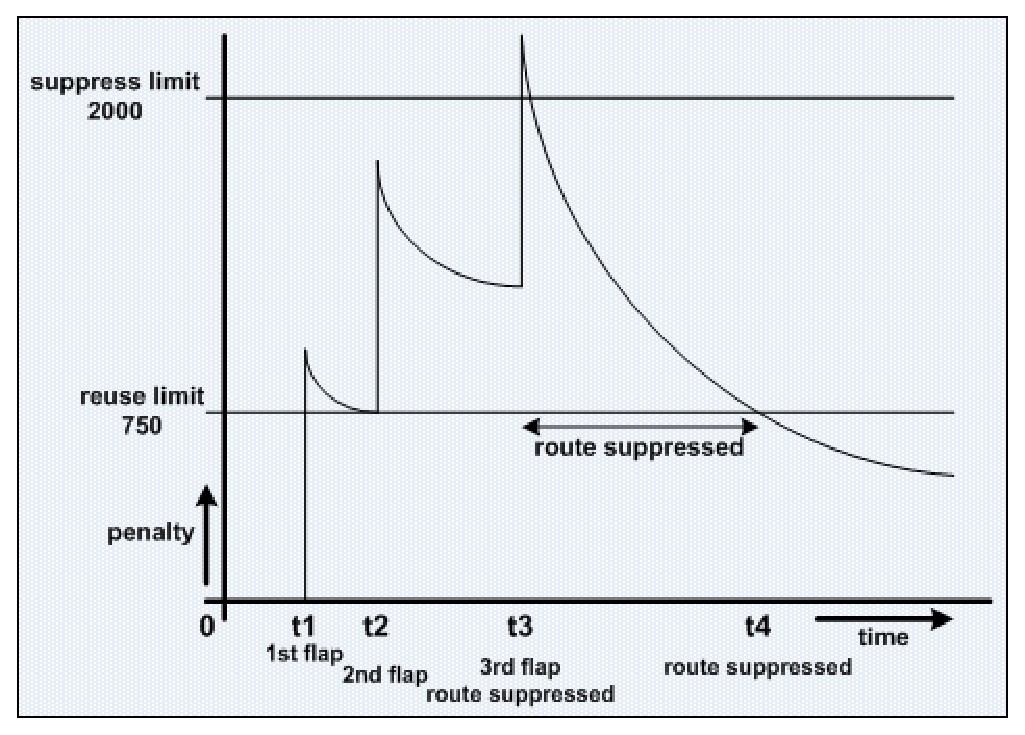
\includegraphics[scale=0.5]{route_damping} 
\par\end{center}

Penalty terms are re-computed at regular time intervals using timers.
Also, every time an update for a route is received, the penalty term
for that route is re-computed.

The RFC proposes several optimizations to decrease processing time,
at the cost of a slightly bigger memory footprint. \textit{E.g. reuse
lists} are used to not have to recompute the figure of merit of all
routes : damped routes with similar penalty terms are grouped together
in a same reuse list. Penalty terms of the routes in a given reuse
list are then re-computed only when necessary.


\section{Implementation}

Our implementation contains most of the data structure definitions
and functions needed for the route damping algorithm (RFC 2439).
As the RFC leaves little freedom regarding the implementation and the 
design of the data structures, our implementation closely matches the RFC.
The code, along with the list of commits, is publicly available on
{\tt\small https://github.com/alexchap/Albatros-Project}.

Several parts of BIRD had to be modified for the implementation of route damping.
The configuration file parser had to be modified in order to correctly handle the parameters
required by the RFC.
Also, we had to make similar modifications to the command line parser so that suppressed routes
could be listed.
Last but not least, we had to add hooks to BIRD's BGP implementation : whenever a route is added or withdrawn, our code is executed.
Route damping is enabled at configure time by adding the {\tt\small -{}-enable-route-damping}
switch.

\subsection{Data structures}

Data structure details and alternatives are explained in the RFC 2439,
§4.4 (Run Time Data Structures). The main data structure of the implementation
are damping\_config and damping\_info. They can be found in the file
/bird/proto/bgp/damping.h.

The damping\_config structure contains all the BGP configuration parameters
values for one EBGP peer. For instance, this structure carries the
values for the suppressed limit threshold or the reused limit one.
The damping\_info is the structure associated to one route. Therefore,
the figure of merit of the route can be found there as well as the
last time when the penalty of the route has been updated.

An other important structure is the hash table which memorize all
the route of BGP, which name is damping\_info\_fib. This structure
contains all damping\_info structure which has just been describe
here on this subsection. Thus when all the routes must be display
or only a subset of them, this structure damping\_info\_fib must be
retrieved as for instance in the function show\_dampened\_paths in
the file /bird/proto/bgp/damping.c:

A last extremely used structure is the reuse list (reuse\_lists) which
is carried by the damping\_config structure described here above.
The reuse list stores the dampened routes, which are suppressed routes.
It has been implemented in a extremely smart way to mimic the exponential
decay of penalty as shown in section 2 (Overview). Instead of computing
each new penalty value at each new step of the timer, the penalty
of route is reviewed only when it could be potentially under the reuse
threshold and thus, potentially considered as a no-flapping route.
It means that the reuse list system mimics the exponential decay and
tries to find the correct index of the list for each routes. For instance,
a route with a high penalty value will have a more long exponential
decay time before potentially reaching the reuse threshold. Such a
route received a high index (or far from the threshold). It is why
the index could also be seen as a distance metric based on a exponential
curve.

FIBs are provided by BIRD API and implement an hash table that maps IP prefixes to any other data structure, {\tt\small damping\_info}s in our case.
This is an important implementation detail : this hash table indeed establishes a link between routes (\textit{i.e.} IP prefix + {\tt\small bgp\_proto})
and {\tt\small damping\_info}. 

\subsection{Configuration parameters}

Our extended version of BIRD gives network administrators a set of four parameters to control the behaviour of route damping.
In particular, {\tt\small cut\_threshold}, {\tt\small reuse\_threshold}, {\tt\small tmax\_hold} and {\tt\small half\_time} are all modifiable
from the configuration file.
Both {\tt\small tmax\_hold} and {\tt\small half\_time} are expressed in seconds.
Here is an example of configuration :

\begin{verbatim}
protocol bgp bgp_config {
  descriptionl "BGP daemon";
  debug all;

  # Specific config for BGP
  local as 65011;
  source address 10.10.10.11;
  multihop;
  next hop self;
  path metric 1;
 
  # Route damping configuration
  route damping;
  cut_threshold 2500;
  reuse_threshold 1000;
  tmax_hold 3000;
  half_time 900;
}
\end{verbatim}

The {\tt\small route damping} parameters can be used to enable/disable route damping for a particular neighbour.
All the other parameters used by the RFC (\textit{e.g.} decay arrays, scaling factor, ...) are derived from
those four values.

BIRD uses Bison to parse the configuration files and we had to extend it to support the new set of keywords.
Those parameters are passed to the {\tt\small damping\_config\_new} function, which allocates and initializes a new {\tt\small damping\_config} and computes the 
other parameters.

\subsection{Detecting BGP Flapping}

Our implementation sticks to the RFC regarding route flapping detection.
Hooks were added in the BGP module of BIRD for that purpose.
Those hooks ensure that the {\tt\small damping\_add\_route} and {\tt\small damping\_remove\_route} functions get
called as routes are advertised/withdrawn respectively.

As those functions are similar to their equivalent in the RFC, only the relevant implementation details are covered here.
Please refer to the RFC for additional details.

When a route is removed for the first time, a new {\tt\small damping\_info} is allocated in a {\tt\small damping\_info\_fib}, and its penalty term is set to a default value.
The penalty term of this route is updated as the route is re-advertised and removed again.
The penalty term is represented by a scaled integer, so that only the right level of precision is kept during execution.
The main idea is that floating point operations are used when the figure of merit needs to be updated, but the result is stored as an integer (thus saving memory space).
This usually results in an accidental loss of precision, except that in our case, the decrease in precision is controlled so as not to crash the application.
Penalty terms are all implicitely multiplied by 1000, implying that only three digits after the dot are kept.

{\tt\small damping\_info} are de-allocated when the penalty gets smaller than {\tt\small reuse\_threshold} divided by two.
The rationale being that when the penalty term gets much smaller than the {\tt\small reuse\_threshold} index, keeping the {\tt\small damping\_info} structure with a small figure of merit is equivalent to de-allocating it (in the worst ---very unlikely --- case, it will only add the cost of re-allocating a new {\tt\small damping\_info} structure).

\section{Evaluation}

\begin{figure}
\caption{Topology used for our simulation}

\end{figure}

\subsection{Overview}

We used a topology of 27 routers in the NSL cluster in order to evaluate
our implementation. This topology consits of 10 Autonomous systems.
Router number 3 with network prefix 10.0.0.3/24 was the the one that
fed the whole network 10.0.0.0/24 with updates coming from one MRT
dump archive (updates.20100401.1729), that we got from the Route Views
project\cite{routeviews}. This archive corresponds to 15 minutes
of real BGP traffic that were sent by 11 BGP routers. The topology
used is represented in figure x.

We ran 3 simulations and recorded every 10 seconds the total number
of updates and withrawals received from all neighbors for all routers.
When route damping was enabled, we also recorded the number of route
dampened at any given time. 
\begin{enumerate}
\item The first simulation was made without route damping and with the official
bird daemon.... 
\item The seconds was made with our bird implementation and default damping
parameters.... 
\item The third was the same as the second, except for the cut\_threshold
parameters that was set to 1000 instead of 1500.... 
\end{enumerate}

\subsection{Evolution of dampened paths}

\begin{figure}
\caption{Evolution of dampened paths for Simulation 3}

\end{figure}

it represent time vs. the actual number of dampened routes in AS2
(actually, router 3)

also note that we aggregated results for each AS (for better readability)


\subsection{Number of route updates}

\begin{figure}
\caption{Difference of import updates between simulations 1 and 3}

\end{figure}


it's the difference between graph sim1 and graph sim3 -> i.e we have
less updates in SIM3 ! :-)

maybe we can also display one graph with the evolution -> show that
the number is quite huge !! and that's why we show the difference
rather than the two graph on top of each other !


\subsection{Number of withdrawals}

works for sim3, not for sim2 !


\section{Conclusion}

show importance of stability


\section{Future work}

possible extensions

real scale tests


\section{Acknowledgement}

\begin{thebibliography}{6}

\bibitem[1]{rfc2439}The RFC 2439, BGP Route Flap Damping, \href{http://www.ietf.org/rfc/rfc2439.txt}{http://www.ietf.org/rfc/rfc2439.txt}

\bibitem[2]{ripe recommendations} RIPE Recommendations On Route-flap
Damping, \href{http://www.ripe.net/ripe/docs/ripe-378}{http://www.ripe.net/ripe/docs/ripe-378}

\bibitem[3]{bird}Bird Routing Project, \href{http://bird.network.cz}{http://bird.network.cz}

\bibitem[4]{repository}Our publicly available repository, \href{https://github.com/alexchap/Albatros-Project}{https://github.com/alexchap/Albatros-Project}

\bibitem[5]{damping-pic}itcertnotes, \href{www.itcertnotes.com}{http://www.itcertnotes.com}

\bibitem[6]{routeviews}\href{http://routeviews.org}{http://routeviews.org} 

\end{thebibliography}

\end{document}
